\documentclass[12pt,a4paper]{article}
\usepackage[utf8]{inputenc}
\usepackage[russian]{babel}
\usepackage[OT1]{fontenc}
\usepackage{mathtools}
\usepackage{amsfonts}
\usepackage{amssymb}
\usepackage{enumitem}
\usepackage{alltt}
\usepackage{graphicx}
\usepackage{indentfirst}
\usepackage{caption}
\usepackage{float}
\usepackage{wrapfig}
\usepackage{hyperref}
\setlength{\parindent}{0.75cm}
\graphicspath{{pictures/}}
\DeclareGraphicsExtensions{.png}
\usepackage[left=15mm,right=15mm,top=2cm,bottom=2cm]{geometry}
\author{Глотов Алексей}
\begin{document}
\newpage
\begin{center}
\footnotesize{{ГОСУДАРСТВЕННОЕ АВТОНОМНОЕ ОБРАЗОВАТЕЛЬНОЕ УЧРЕЖДЕНИЕ}\break
{ВЫСШЕГО ОБРАЗОВАНИЯ}
\break
{\bf {МОСКОВСКИЙ ФИЗИКО-ТЕХНИЧЕСКИЙ ИНСТИТУТ}}
\break
\small{(НАЦИОНАЛЬНЫЙ ИССЛЕДОВАТЕЛЬСКИЙ УНИВЕРСИТЕТ)}}
\break
\hfill \break
\hfill \break
\begin{center}
\large{Кафедра общей физики}
\end{center}
\hfill \break
\hfill \break
\hfill \break
\hfill \break

\begin{center}
\large{Вопрос по выбору}
\end{center}
\hfill \break\\
\LARGE{Дробовой шум}
\end{center}
\hfill \break
\hfill \break
\hfill \break
\hfill \break
\hfill \break
\hfill \break
\hfill \break
\hfill \break
\hfill \break
\hfill \break
\begin{flushright}
\large Обучающийся: Глотов А.А
\end{flushright}
\hfill \break
\hfill \break
\hfill \break
\hfill \break
\hfill \break
\hfill \break
\hfill \break
\hfill \break
\hfill \break
\hfill \break
\hfill \break
\hfill \break
\hfill \break
\begin{center}
Долгопрудный \break
 2022
\end{center}
\thispagestyle{empty}
\newpage

\section{Введение}
\subsection{Аннотация}

\par Данная работа посвящена изучению эффекта Шоттки (дробовой шум) при прохождении тока через анодную лампу, подключенную параллельно колебательному RLC-контуру.
\break

\textbf{Цели работы: }\begin{enumerate}
\item Измерение заряда электрона по дробовому шуму 

\item Определить правомерность используемых в теоретической части допущений и соответствие теории и эксперимента
\end{enumerate}

\textbf{В работе используются: } стенд для измерения дробового шума, состоящий из шумового диода, блока питания, широкополосного усилителя, квадратичного детектора и кварцевого генератора синусоидальных колебаний.


\subsection{Теоретические сведения}

\par Дробовой шум — беспорядочные флуктуации числа частиц относительно их среднего значения связанные с их дискретностью. Для электрически заряженных частиц — электронов, ионов проявляется как флуктуации токов в электрических цепях и электрических приборах. Перемещение каждого носителя заряда в цепи через воображаемую поверхность секущую провод сопровождается всплеском тока в цепи, обусловленного дискретностью носителей электрического заряда. Эффект был предсказан Шоттки в 1918 году и носит его имя. В повседневной жизни проявляется в виде акустического шума в динамике радиоприёмника (похожего на шум рассыпающейся дроби, в честь чего был назван), в виде "снега" на экране телевизора и т.п. Также это один из немногих способов измерения абсолютного заряда электрона, наряду с опытом Милликена и электролизом. Флуктуации анодного тока — при заданной его величине — пропорциональны заряду электрона, поэтому, исследуя их, можно измерить заряд электрона. 

\par Дробовой шум, наряду с тепловым шумом, является принципиально неустранимым шумом, как вызванный дискретностью электрического заряда электрона. В связи с этим данные шумы являются тем пределом, ниже которого невозможно ослабить шумы в электрических приборах.

\par Для диода, работающего в режиме насыщения, дробовой шум описывается с помощью модели импульсного случайного процесса. Протекающий в цепи ток I(t) представляется в виде суперпозиции отдельных импульсов: I(t) = $\sum_k I_k(t - t_k)$, $t_k$ случайный момент появления импульса, $I_k(t) = I_0(t)$ - прямоугольный сигнал с максимальным значением $I_0$

\par Ввиду независимости импульсов, процесс прохода одиночных электронов описывается распределением Пуассона, то есть среднее значение анодного тока I и дисперсия его флуктуаций описывается как 

\begin{equation}
I = \nu\int_{-\infty}^{\infty}{I_0(t)dt} \;\;\;\;\;\;\; \sigma_I^2 = \nu\int_{-\infty}^{\infty}{I_0^2(t)dt}
\end{equation}
где $\nu$ - средняя частота импульсов

\par $s_\text{др}$ - спектральная плотность дробового шума определяется как 

\begin{equation}
s_\text{др}(f) = 2\nu{F^2(t)} = 2\nu(\int_{-\infty}^{\infty}{I_0(t)*\exp{-2\pi{i}ft}dt})^2
\end{equation}

\par Проинтегрировав выражение, считая, что $\Delta{f}$ - мал (то есть время исследования достаточно велико), а также понимая, что импульс тока обеспечивается прохождением одиночного электрона, получим $s_\text{др} = 2Ie$

\par Или средний ток дробового шума: $I_\text{др}^2=2eI\Delta{f} $ 

\par Добавим также, что при использовании лампового диода (в т.ч. в данной работе), предыдущая формула может принять вид $I_\text{др}^2=2KeI\Delta{f}$, где K - коэффициент подавления дробового шума пространственным зарядом (K < 1). Такое возможно, если диод работает не в режиме насыщения.

\subsection{Схема эксперимента}

\par Рассмотрим, как меняется во времени ток, проходящий во внешней цепи электронной лампы (диода), при движении через неё отдельного электрона. Пока из катода не вылетит электрон, тока в цепи лампы нет. Ток появляется, когда электрон покидает катод, и кончается, когда он приходит на анод. Распределение этого тока во времени носит сложный характер, зависящий от геометрии электродов, от распределения потенциалов в межэлектродном пространстве и от скорости электронов.

\begin{wrapfigure}[12]{r}{0.15\textheight}
	\vspace{-4ex}
	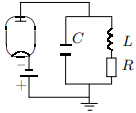
\includegraphics[width=4cm, height=4cm]{VPV-3_1}
	\caption{Схема включения колебательного контура}
	\label{img1}
\end{wrapfigure}	 

\par В дальнейшем нас не будет интересовать форма токового импульса. Нам достаточно знать, что этот импульс является очень кратковременным ($\thicksim 10^{-8}$ с) и что за время этого импульса 
$\int{Idt} = e$, где e — заряд электрона. Будем рассматривать режим насыщения диода, когда пространственный заряд в межэлектродном пространстве отсутствует и анодный ток зависит только от количества электронов, испущенных катодом. 

\par Для обнаружения дробового шума в анодную цепь лампы включена нагрузка — параллельный колебательный контур (рис. 1). Токовый импульс, связанный с прохождением электрона через диод, приводит к зарядке конденсатора C входящего в состав RLC контура, что — в зависимости от фазы колебаний контура — усиливают или ослабляют колебательный процесс, амплитуда и фаза которого случайным образом меняются во времени. Кроме заряда, связанного с колебательным процессом, на конденсаторе также есть заряд, возникающий из-за наличия среднего тока, но он нас интересовать не будет. Установившееся значение амплитуды определяется тем, что средняя энергия, которую приносят электроны на конденсатор, равна энергии, которая рассеивается в колебательном контуре.

\par Пусть при электрических колебаниях в контуре мгновенное значение напряжения на конденсаторе равно

\begin{equation}\label{U}
U = U_0\cos\omega{t}
\end{equation}

\par Для пролёта очередного электрона заряд на конденсаторе равен $q_1 = CU_0\cos\omega{t}$, а после пролёта он принимает значение $q_2$:

\begin{equation} \label{q2}
q_2 = q_1 + e = CU_0\cos\omega{t} + e
\end{equation}

\par Рассчитывая энергию конденсатора по формуле 

\begin{equation}\label{W}
W = \frac{q^2}{2C}
\end{equation} 

найдем, что приход электрона увеличивает энергию конденсатора на $\Delta{W}$:

\begin{equation}\label{dW}
\Delta{W} = \frac{q_1^2-q_2^2}{2C} = \frac{2eCU_0\cos\omega{t} + e^2}{2C}
\end{equation}

\par Пусть в секунду через лампу проходят N электронов. Полное увеличение средней энергии конденсатора складывается из N слагаемых, определяемых формулой (\ref{dW}). При этом вклад от первого члена формулы обращается в нуль, так как электроны приходят на конденсатор в произвольные моменты времени, а среднее значение $\cos\omega{t}$ равно нулю. Средняя мощность, приносимая электронами на конденсатор, определяется поэтому только вторым слагаемым и равна

\begin{equation}\label{P}
P = N\frac{e^2}{2C}
\end{equation}

\par Рассчитаем теперь потери в сопротивлении. Проходящий через него ток $I_R$ складывается из постоянного тока $I_=$ и колебательного тока контура $I_\thicksim$. Выделяемая в сопротивлении мощность в среднем равна 

\begin{equation}\label{P_R}
<P_R> = <I^2R> = R<(I_= + I_\thicksim)^2>
\end{equation}

\par Переменная составляющая тока может быть выражена через напряжение на конденсаторе:

\begin{equation}\label{I_a}
I_\thicksim = \frac{dq}{dt} = -CU_0\omega\sin\omega{t}
\end{equation}

\par Подставим \ref{I_a} в \ref{P_R}, возведем сумму $I_=$ и $I_\thicksim$ в квадрат и усредним результат по времени. Средние значения $<\sin\omega{t}> = 0$, $<\sin^2\omega{t}> = 1/2$, откуда 

\begin{equation}\label{P_R}
<P_R> = RI_=^2 + R<I_\thicksim^2> = RI_=^2 + \frac{1}{2}RC^2U_0^2\omega^2
\end{equation} 

\par Таким образом, мощность, выделяемая на сопротивлении R, - это мощность, которую выделяют в нем постоянный ток диода и ток колебаний, возникающий в контуре из-за дробового шума.
\par Приравниваем мощность \ref{P}, возбуждаемую электронами в контуре, к мощности $R<I_\thicksim^2>$, теряемой на сопротивлении из-за наличия колебаний: 

\begin{equation}\label{9}
N\frac{e^2}{2C} = \frac{1}{2}R(CU_0\omega)^2
\end{equation}

\par Отметим, что $Ne = I_a$, а амплитудное значение напряжения на конденсаторе $U_0$ связано с эффективным значением $U_\text{эфф}$ соотношением $U_\text{эфф}^2 = \frac{U_0^2}{2}$, найдем для заряда электрона e следующую формулу:

\begin{equation}\label{e}
e = \frac{2\omega^2C^3RU_\text{эфф}^2}{I_a}
\end{equation}

\par Таким образом, измеряя ток $I_a$, проходящий через диод, и среднеквадратичное напряжение шума на контуре $U_\text{эфф}^2$, можно определить заряд электрона. Формула \ref{e} может быть записана через добротность контура. Как известно, добротность контура Q связана с его параметрами формулой 

\begin{equation}\label{Q}
Q = \frac{1}{\omega{RC}}
\end{equation} 

\par Окончательная формула для расчета заряда электрона имеет вид 

\begin{equation}\label{e_fin}
e = \frac{2\omega{C^2}U_\text{эфф}^2}{I_aQ}
\end{equation}

\subsection{Экспериментальная установка}

\par Блок-схема установки изображена на рис. 2. В качестве шумового диода используется диод 2Д3Б, работающий в режиме насыщения. В его анодную цепь включён параллельный колебательный контур LC. Активное сопротивление катушки L играет роль резистора
R. Конденсатор C непосредственно включён в цепь контура при нижнем положении переключателя $" U_\text{к} "$ (его кнопка не нажата). Измерение напряжения на контуре производится квадратичным детектором. Перед измерениями сигнал, поступающий с контура, усиливается усилителем.

\begin{figure}[H]
	\begin{center}
		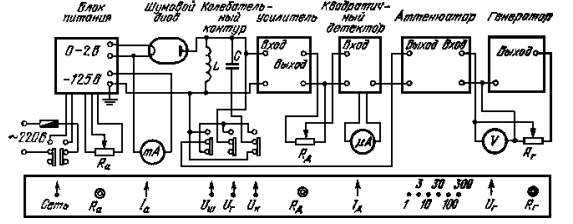
\includegraphics[width=15cm, height=5cm]{VPV-3_2}
	\end{center}
	\centering \caption{Блок-схема установки для измерения дробового шума. Внизу изображена нижняя часть передней панели с ручками и кнопками управления}
	\label{img2}
\end{figure}

\par Усилитель и квадратичный детектор используются не только для измерения шумовых колебаний контура, но и для других целей. При измерении шумов важно, чтобы на усилитель не попали колебания с генератора, изображённого в правой части схемы. Для этого лучше всего заземлить выход аттенюатора. Это делается нажатием кнопки $" U_\text{ш} "$, что соответствует на схеме рис. 2 переводу его переключателя в верхнее положение.

\par Сила анодного тока шумового диода в режиме насыщения определяется эмиссией (а значит, температурой) его катода. Анодный ток $I_a$ измеряется миллиамперметром и регулируется потенциометром $R_a$, ручка которого на панели прибора обозначена $" R_a "$. Чувствительность измерительной схемы регулируется делителем напряжения $R_\text{д}$, расположенным между усилителем и квадратичным детектором. Его ручка на панели обозначена $" R_\text{д} "$. На выходе квадратичного детектора установлен микроамперметр. Отклонение стрелки микроамперметра пропорционально квадрату напряжения на входе детектора, поэтому он пригоден для измерения переменных напряжений. Таким образом, показания микроамперметра пропорциональны квадрату шумового напряжения, причём коэффициент пропорциональности зависит от положения реостата $R_\text{д}$ и, вообще говоря, неизвестен. Поэтому при измерениях экспериментатор замечает показание микроамперметра, а затем вместо сигнала с колебательного контура подаёт на вход усилителя калибровочный сигнал с настроенного на ту же частоту генератора. Этот сигнал измеряется вольтметром (обозначение $" U_\text{г} "$ на панели) и ослабляется в точно известное число раз прецизионным аттенюатором. При измерениях напряжение на генераторе подбирается так, чтобы стрелка микроамперметра вернулась к отмеченному делению. В этом случае напряжение шумов равно известному напряжению, подаваемому на усилитель с аттенюатора. Делитель $R_\text{д}$ во время этой процедуры, конечно, нельзя трогать.

\par Генератор используется не только для калибровки квадратичного детектора, но и для измерения добротности контура. Измерения производятся по методу Q-метра. Включим в контур генератор Г (настроенный на собственную частоту контура), как это изображено на рис. 3. Найдём напряжение $U_\text{к}$, подаваемое на усилитель и измеряемое квадратичным детектором:

\begin{center}
$U_\text{к} = U_r - \frac{1}{i\omega{C}} = U_r - \frac{U_r}{i\omega{RC}} \approx \frac{iU_r}{\omega{RC}}$
\end{center}

\par При написании последнего равенства считалось, что контур обладает высокой добротностью, $Q = \frac{1}{\omega{RC}} \gg 1$. Заменяя $\frac{1}{\omega{RC}}$ через добротность контура, найдем 

\begin{equation}\label{Q_fin}
Q = \frac{|U_\text{к}|}{|U_r|}
\end{equation}

\par Итак, для измерения добротности контура нужно сравнить напряжение на генераторе с напряжением на катушке самоиндукции. Напряжение на генераторе $U_\text{г}$ измеряется вольтметром генератора (рис. 2). Измерение напряжения на катушке самоиндукции не так просто. 

\begin{wrapfigure}[11]{r}{0.25\textheight}
	\vspace{-4ex}
	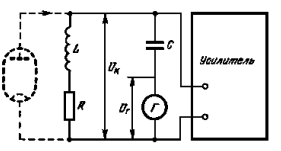
\includegraphics[width=7cm, height=4cm]{VPV-3_3}
	\centering \caption{Схема для измерения
добротности колебательного контура}
	\label{img3}
\end{wrapfigure}	 

\par При измерении напряжения $U_\text{г}$, создаваемого генератором на катушке самоиндукции, необходимо учитывать и шумовое напряжение $U_\text{ш}$, имеющееся на катушке. Это напряжение при измерениях продолжает возбуждаться диодом, так как при измерениях добротности контура диод находится в рабочем режиме. Отключить диод при измерении нельзя, поскольку добротность контура от этого заметно изменится: при измерениях шума контур шунтирован диодом, что снижает его добротность; в этом положении и должна измеряться добротность контура. При включении генератора в контур на вход усилителя сумма $U_\text{к}$ и $U_\text{ш}$. При этом ток детектора $I_\text{д}$ пропорционален $<(U_\text{ш} + U_\text{к})^2>$. Сдвиг фаз между колебаниями $U_\text{ш}$ и $U_\text{к}$ непрерывно изменяется. Поэтому

\begin{center}
$I_\text{д} \varpropto <(U_\text{ш} + U_\text{к})^2> = <U_\text{ш}^2> + 2<U_\text{ш}U_\text{к}> + <U_\text{к}^2>$
\end{center}
в то время как до включения генератора ток детектора был пропорционален $U_\text{ш}^2$

\begin{figure}[H]
	\begin{center}
		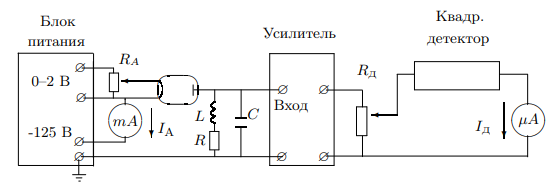
\includegraphics[width=15cm, height=5cm]{VPV-3_4}
	\end{center}
	\centering \caption{Схема для измерения напряжения шума}
	\label{img4}
\end{figure}

\par Таким образом, $U_\text{к}^2$ приращение тока квадратичного детектора, происходящему при включении напряжения $U_\text{г}$. Чтобы подставить это приращение в формуле \ref{Q_fin}, оно должно быть пересчитано в напряжение генератора. Это делается следующим образом. Нужно заметить показание квадратичного детектора при нулевом напряжении на выходе генератора. Затем нужно становить на выходе генератора некоторое напряжение $U_\text{г}$ и зафиксировать приращение тока детектора $\Delta{I_\text{д}}$, вызванное напряжением генератора. После этого вместо колебательного контура на вход усилителя следует подключить генератор с аттенюатором. Сигнал с генератора и положение аттенюатора нужно подобрать таким образом, чтобы показание микроамперметра было равно измеренному ранее приращению $\Delta{I_\text{д}}$. Показание вольтметра генератора равно искомому напряжению $U_\text{к}$ 

\begin{figure}[H]
	\begin{center}
		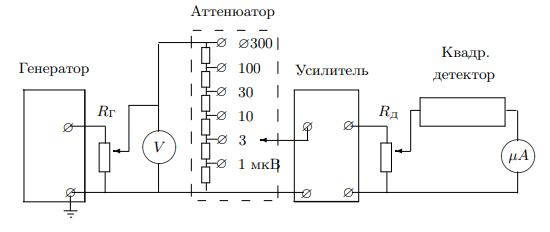
\includegraphics[width=15cm, height=5cm]{VPV-3_5}
	\end{center}
	\centering \caption{Схема для измерения напряжения на генераторе}
	\label{img4}
\end{figure}


\newpage

\section{Ход работы}
\subsection{Проверка квадратичности детектора}
	
	\par Установим квадратичность детектора, с которого будем снимать значения напряжений. Для этого снимем зависимость I(U) и определим проверим линейность $I(U^2)$

\begin{center}
	\begin{tabular}{|c|c|c|c|c|c|c|c|c|c|c|c|c|c|c|c|c|c|c|c|c|c|c|c|}
	\hline 
	U, мкВ & 30 & 34 & 40 & 44 & 48 & 52 & 56 & 60 & 62 & 66 & 68 & 70  \\ 
	\hline 
	I, мкА & 10 & 14 & 18 & 22 & 26 & 30 & 34 & 38 & 42 & 46 & 50 & 54   \\ 
	\hline 
	$U^2$, мкВ$^2$  & 900 & 1156 & 1600 & 1936 & 2304 & 2704 & 3136 & 3600 & 3844 & 4356 & 4624 & 4900   \\ 
	\hline 
	U, мкВ & 74 & 76 & 78 & 80 & 82 & 84 & 86 & 88 & 90 & 92 & 96 \\ 
	\hline 
	I, мкА & 58 & 62 & 66 & 70 & 74 & 78 & 82 & 86 & 90 & 94 & 100 \\ 
	\hline 
	$U^2$, мкВ$^2$  & 5476 & 5776 & 6084 & 6400 & 6724 & 7056 & 7396 & 7744 & 8100 & 8464 & 9216 \\ 
	\hline 
	\end{tabular} 
\end{center}

\par $\Delta{U} = 2$мкВ,    $\Delta{I} = 2$мкА

\begin{figure}[H]
	\begin{center}
		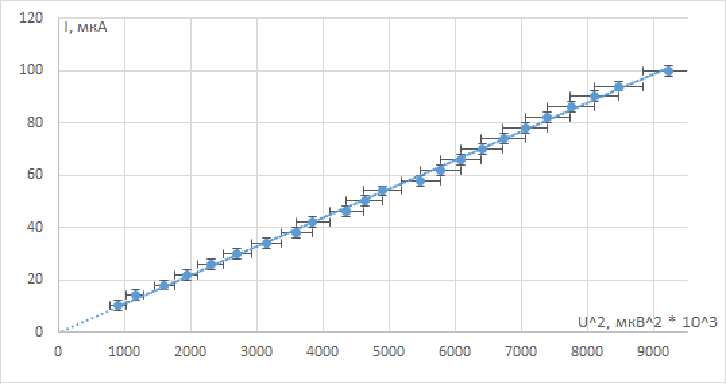
\includegraphics[width=18cm, height=8cm]{VPV-3_gr_1}
	\end{center}
	\centering \caption{Проверка квадратичности детектора}
	\label{gr1}
\end{figure}

\par $I = (0.011*U^2 + 0.0078)$ мкА

\par $\sigma_{k} = 0,9*10^{-4}\frac{\text{мкА}}{\text{мкВ}^2}$, $\varepsilon_{k} = 4\%$, $\sigma_{b} = 0,4*10^{-2}\text{мкА}$

\par Видим, что значение b = 0 лежит в пределах $\sigma_{b}$, значит, с высокой вероятностью, 0 - истинное значение b. Вместе с 
малой погрешностью k, в основном обуславливающейся приборной погрешностью, можно говорить о подтверждении квадратичности детектора

\par Перейдем к основной части нашей работы. Пошагово выполним действия, приведенные в п. 1.4 в частях II и III. Будем повторять изменения при одинаковых параметрах до 5 раз и усреднять значения (при наличии расхождений)

\subsection{Измерение напряжения шума}

\par Внесем полученные данные в таблицу. Повторим эксперимент при различных чувствительностях квадратичного детектора, чтобы убедиться в отсутствии влияния этого параметра на результат

\begin{tabular}{|p{0.15\linewidth}|p{0.1\linewidth}|p{0.1\linewidth}|p{0.1\linewidth}|p{0.1\linewidth}|p{0.1\linewidth}|p{0.1\linewidth}|}
  \hline 
  \multicolumn{7}{|c|}{$I_a$ = 1.0 мА} \\ 
  \hline 
  $I_\text{д}$, мА & 50 & 40 & 58 & 44 & 36 & 54 \\ 
  \hline 
  $U_\text{эфф}$, мкВ & 74 & 72 & 74 & 72 & 72 & 74 \\ 
  \hline 
  \multicolumn{7}{|c|}{$I_a$ = 2.0 мА} \\ 
  \hline 
  $I_\text{д}$, мА & 40 & 50 & 60 & 70 & 80 & • \\ 
  \hline 
  $U_\text{эфф}$, мкВ & 100 & 100 & 100 & 100 & 100 & • \\ 
  \hline 
  \multicolumn{7}{|c|}{$I_a$ = 3.0 мА} \\ 
  \hline 
  $I_\text{д}$, мА & 40 & 50 & 50 & 70 & 80 & • \\ 
  \hline 
  $U_\text{эфф}$, мкВ & 120 & 120 & 120 & 120 & 120 & • \\ 
  \hline 
  \multicolumn{7}{|c|}{$I_a$ = 4.0 мА} \\ 
  \hline 
  $I_\text{д}$, мА & 40 & 50 & 60 & 70 & 80 & • \\ 
  \hline 
  $U_\text{эфф}$, мкВ & 130 & 130 & 130 & 130 & 140 & • \\ 
  \hline 
  \end{tabular}   

\subsection{Определение добротности контура}

\par Для различных чувствительностей детектора и различных значений тока $I_a$ проведем серию измерений для определения Q и посчитаем заряд электрона, по результатам каждой серии измерений. В качестве значения генератора возьмем усредненные значения из п. 2.2

\begin{center}
\begin{tabular}{|c|c|c|c|c|c|c|c|}
\hline 
$I_1$, мкА & $I_2$, мкА & $U_1$, мкВ & $\Delta{I}$, мкА & $U_2$, мкВ & Q & e, Кл*$10^{-19}$ & $\Delta{e}$, Кл*$10^{-19}$\\ 
\hline 
\multicolumn{7}{|c|}{$I_a$ = 1,0 мА, $U_\text{эфф}$ = 73 мкВ} \\ 
\hline 
72 & 100 & 0,26 & 28 & 56 & 215 & 1,02 & 0.07 \\ 
\hline 
60 & 90 & 0,32 & 30 & 62 & 194 & 1,07 & 0.07 \\ 
\hline 
30 & 62 & 0,5 & 32 & 88 & 176 & 1,25 & 0.07 \\ 
\hline 
20 & 48 & 0,7 & 28 & 100 & 143 & 1,46 & 0.08 \\ 
\hline 
40 & 80 & 0,54 & 40 & 86 & 159 & 1,31 & 0.07 \\ 
\hline 
50 & 94 & 0,5 & 44 & 85 & 170 & 1,30 & 0.07 \\ 
\hline 
\multicolumn{7}{|c|}{$I_a$ = 2,0 мА, $U_\text{эфф}$ = 100 мкВ} \\ 
\hline 
20 & 32 & 0,66 & 12 & 79 & 120 & 1,68 & 0.06 \\ 
\hline 
30 & 54 & 0,72 & 24 & 140 & 194 & 1,03 & 0.03 \\ 
\hline 
40 & 70 & 0,7 & 30 & 140 & 200 & 1,01 & 0.03 \\ 
\hline 
50 & 90 & 0,7 & 40 & 98 & 140 & 1,44 & 0.05 \\ 
\hline 
60 & 90 & 0,5 & 30 & 77 & 154 & 1,44 & 0.05 \\ 
\hline 
\multicolumn{7}{|c|}{$I_a$ = 3,0 мА, $U_\text{эфф}$ = 120 мкВ} \\ 
\hline 
20 & 30 & 0,76 & 10 & 82 & 108 & 1,79 & 0.05 \\ 
\hline 
30 & 50 & 0,86 & 20 & 97 & 113 & 1,71 & 0.04 \\ 
\hline 
40 & 70 & 0,9 & 30 & 105 & 117 & 1,65 & 0.04 \\ 
\hline 
50 & 90 & 0,96 & 40 & 110 & 115 & 1,68 & 0.04 \\ 
\hline 
60 & 90 & 0,64 & 30 & 88 & 137,5 & 1,40 & 0.03 \\ 
\hline 
\multicolumn{7}{|c|}{$I_a$ = 4,0 мА, $U_\text{эфф}$ = 132 мкВ} \\ 
\hline 
20 & 80 & 2,7 & 60 & 235 & 87 & 2,61 & 0.08 \\ 
\hline 
30 & 90 & 2,1 & 60 & 190 & 90 & 2,50 & 0.08\\ 
\hline 
40 & 80 & 1,3 & 40 & 140 & 108 & 2,10 & 0.09\\ 
\hline 
50 & 80 & 0,84 & 30 & 105 & 125 & 1,95 & 0.04 \\ 
\hline 
60 & 90 & 0,9 & 30 & 96 & 107 & 2,46 & 0.05\\ 
\hline 
\end{tabular} 
\end{center}

Основываясь на \ref{e_fin} определим формулу подсчета погрешностей:

\begin{center}
$\varepsilon_{e} = \sqrt{2*\varepsilon({U_{\text{эфф}}})^2+\varepsilon({I_{a}})^2+\varepsilon({U_1})^2+\varepsilon({U_2})^2}$
\end{center}

Приборные погрешности примем равными : $\Delta{I_a}$ = 0,05 мА,  $\Delta{U} = 0.01/0.05/1$ мкВ для пределов измерения 1/3/100 мкВ соответственно, $\Delta{I_{12}}$ = 0.2 мкА

\par Итоговое значение e получим усреднением : $(1,60 \pm 0,06)*10^{-19}$ Кл, $\varepsilon_e = 4\%$ 

\section{Обсуждение результатов}


\par Вернемся к сделанному при написании формулы \ref{q2} предположению о том, что при прохождении электрона через диод заряд конденсатора и, следовательно, его энергия возрастают мгновенно. Как ясно из вывода, это предположение не приводит к ошибкам, если аргумент косинуса в \ref{q2} за время прохождение токового импульса меняется незначительно. Уже упоминалось, что время пролета электрона через диод $\tau$ по порядку величины равно $10^{-8}$ c. Контур настроен на частоту $f \simeq 10^5$ Гц. Следовательно, 

\begin{center}
$\omega\tau = 2\pi{f}\tau \simeq 2\pi\cdot{10^5}\cdot{10^{-8}} \approx 10^{-2} \ll 1$
\end{center}

\par При измерении напряжении шума мы получили ожидаемый результат: получаемое эффективное напряжение шумов зависит только от тока на аноде нашего диода и не зависит от чувствительности. Калибровка детектора повлияла на численные показания, но итоговые значения не менялись (в пределах погрешности), т.к. это независимые друг от друга системы

\par При подсчете значений e наблюдается явная тенденция роста значения e с ростом $I_a$, которой не должно быть. Причем тенденция продолжается, не остановившись на истинном значении электрона (ближе всего оказалась серия измерений при $I_\text{д}$ = 3 мА). Это позволяет выдвинуть теорию о том, что значение C и/или $\omega$ было дано завышенным. Возвращаясь к полученным значениям, можно почти однозначно утверждать о наличии коэффициента K, отличного от 1. Причем он прогнозируемо уменьшается с ростом $I_\text{к}$ (нагрев катода приводит к тому, что электроны срываются с большей энергией, то есть влияние пространственного заряда уменьшается). 
\par О расхождении экспериментального значения и истинного, составившего менее одного процента, можно сказать, что при выборе других настроечных параметров ($I_\text{k}$), соответствие оказалось бы сильно хуже. Достаточно малая величина экспериментальной погрешности и большой разброс значений даже в пределах одной и той же серии измерений говорит о наличии неучтенных в изначальной теории параметров или значительном влиянии случайных внешних событий. В пользу этой теории то, что повторные измерения, сделанные сразу же, совпадают с остальными результатами. Повторенные же через некоторое время (в данном случае - неделя) измерения могут существенно различаться, но совпадать между собой

\end{document}

